% Chapter 4

\chapter{Results}

\label{Chapter4}

We begin our discussion of the results with preliminary analysis of the data that helped shape the experimental design. Here we seek to understand what are some of the overarching patterns in music listening habits and how these look at an individual level.

After this we present a summary of our results followed by a discussion of the performance of each individual method.

\section{Preliminary analysis}

\subsection{Daily play patterns}

By grouping track plays into 30 min intervals and aggregating by periods within a day, we see a clear daily pattern with music listening hitting a peak at around 5pm and a trough at around 6am.

\begin{figure}[h!]
	\centering
	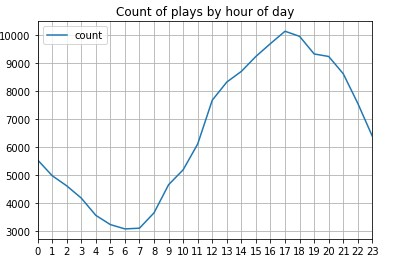
\includegraphics[width=7cm, keepaspectratio,]{fig004.jpg}
	\caption{5-5.30pm is peak listening time}
	\label{3a}
\end{figure} 

Zooming out to view the pattern across an entire week in figure \ref{3b}, we see that the daily pattern occurs across every day of the week with weekends having a lower total number of plays.

\begin{figure}[h!]
	\centering
	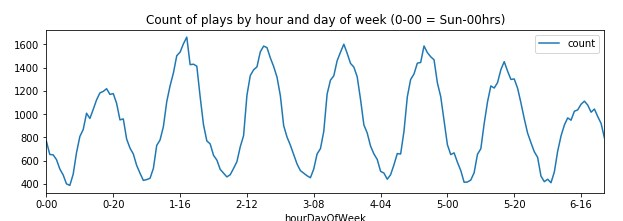
\includegraphics[width=7cm, keepaspectratio,]{fig005.jpg}
	\caption{Most popular times to listen to music across all users}
	\label{3b}
\end{figure} 

At a high level therefore one can get good accuracy by simply anticipating music demand to peak at 5pm. However if we select two users at random, we see (see fig. \ref{3c}) that these daily patters are not as strongly discernable. This demonstrates why models modeling the high levels patterns is not enough for individual user prediction. 

\begin{figure}[h!]
	\centering
	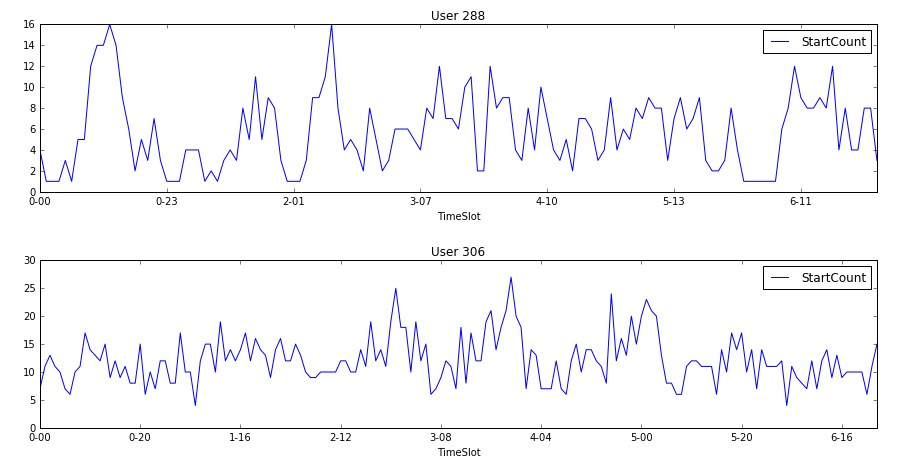
\includegraphics[width=7cm, keepaspectratio,]{fig006.jpg}
	\caption{Most popular times to listen to music by individual user}
	\label{3c}
\end{figure} 

\subsection{Inter-event times}

The dataset contains a timestamp associated with each user. This does not necessarily mean the user played a song in its entirety. Analysis shows plenty of cases where the interval time between tracks was a few seconds suggesting the user skipped tracks. 

Figure \ref{3d} shows a frequency plot of intervals. Intervals beyond 30 minutes continue the exponential decrease and are not shown. We see that while the mode is on par with a typical song length, there is a significant number of plays that lasted under 5 minutes. 

\subsection{Time-series analysis}

Here we examine our data once it has been transformed in a binary sequence of events (1) and non-events(0). We seek to understand better how an optimizer may perform based on traits of the data.

We begin with assessing how well our baseline model may perform based on assuming $t = t-1$. Fig \ref{fig12} shows that the 76\% of Plays, also had a play in t-1. However simply using this as a rule would also capture 2.2\% of non-plays.

\begin{figure}[h!]
	\centering
	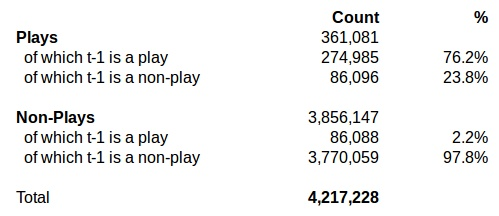
\includegraphics[width=7cm, keepaspectratio,]{fig012.jpg}
	\caption{}
	\label{fig12}
\end{figure} 

Furthermore the 23.8\% of Plays that did not have a Play in the prior period are harder to predict yet of more interest as they representthe beginning of the listneing period and therefore more useful to a music recommender system. 

Given the daily patterns we have seen, it might be reasonable to assume that looking at the same period 24 hours prior may be a good indicator of whether t is a play event. However as we see from fig. \ref{fig12b} this is not a reliable indicator either.

\begin{figure}[h!]
	\centering
	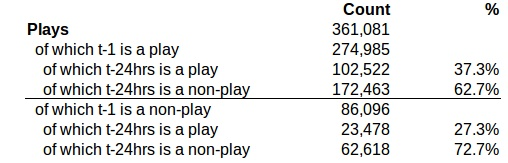
\includegraphics[width=7cm, keepaspectratio,]{fig012b.jpg}
	\caption{}
	\label{fig12b}
\end{figure} 

What both of these results tell us is that fairly high precision score of around 76\% ought ot be possible purely based on t-1 but going above this while having a good precision score on the non-play events will be harder.

Finally it was found that of rows where all timelags had a non-play event, 0.62\% of rows had a play event. As this was a low number it was deemed safe to remove all such rows from the dataset in order to improve the speed and quality of analysis. 

\subsection{Outliers}

The data was checked for any unusual outliers that may impinge upon the goal of developing a model to predict user behaviour. An analysis of plays by user reveals a high amount of variance between users on how many tracks are played. 

\begin{figure}[h!]
	\centering
	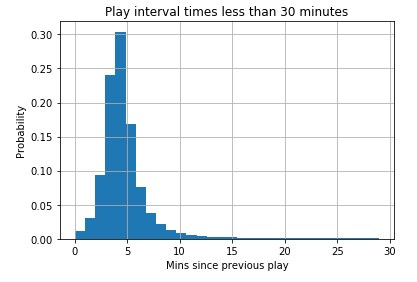
\includegraphics[width=7cm, keepaspectratio,]{fig003.jpg}
	\caption{}
	\label{3d}
\end{figure} 

For our purposes these are include as evidence that the user was interested in playing music at time $t$ and therefore treated as a Play event.

We can also assume that the song plays are not independent of one another, in that the probability of a play event at time t+1 is significantly higher if there was an event at time t. 

\newpage

Further analysis showed one user in particular with very high amount of plays, with very low durations, suggesting it was likely to have been generated by a bot, possibly a LastFM test. This was excluded from the dataset.

\begin{figure}[h!]
	\centering
	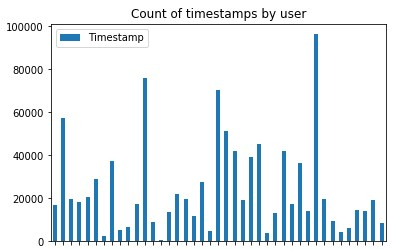
\includegraphics[width=7cm, keepaspectratio,]{fig002.jpg}
	\caption{Total play count by user}
	\label{fig2}
\end{figure} 


\section{Main results} % Methodology

\subsection{Summary}

Fig. \ref{fig13a} shows the results from our experiments. We see how that the baseline model scores highly on precision but low on recall. In other words assuming $t = t-1$ is often quite often correct given that a group of songs are often played consecutively, but it fails to pick up the start and end points of a sequence of song plays, hence the lower recall.

\begin{figure}[h!]
	\centering
	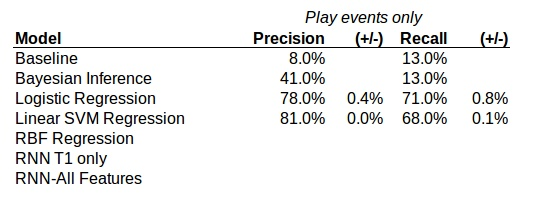
\includegraphics[width=8cm, keepaspectratio,]{fig013b.jpg}
	\caption{Summary of results. Note that both RNN models included non-time lag features (e.g. IsMon)}
	\label{fig13b}
\end{figure}  

The Bayesian Inference model performed poorly on both measures. This would suggest that the difference between the population patterns and what is observed at an individual level differs too much for the prior probability to be accurate for any one individual user. However this does not rule necessarily rule out the Bayesian approach. An improvement might be to apply a logistic regression model in which the weights are continually updated with each new observation from the user. However such as an approach was not looked at in this research.

Our remaining models exhibit the tension between achieving a good accuracy and achieving a good recall. The Logistic regression model performs below average on precision but is second highest on recall. The Linear SVM and RMF regression models are on par with one another with the former achieving the highest score on prevision, and the latter on recall. 

The Linear SVM model ignores probabilities that fall within a margin of the decision boundary during its optimization process. That this translates into performing well on precision may be due to placing lesser emphasis on ad-hoc play events that aren't indicative of a users general behaviour, as these probablities would likely fall near the decision boundary. Alternatively it could be better at dealing with the first play of a sequence whereby if often, but not always occurs at the same time each day; again leading to probabilities nearer the decision boundary.

The RBF model generally performs well on both metrics. Note that the RBF classifciation was restricted to 100k rows of training data as it was found the computational cost of 500k rows was too high so it had less training data to work with than the Linear SVM. The high recall rate of 68\% indicates that inputs have a non-linear relationship to the output and that this is especially helpful to predicting the start and end of a play sequence as seen by the high recall score. 
 
The RNN models were trained on 50k rows of data due to the computational cost of evaluating a large number of hyperparameters. Two types of models were tested - one with $t-1$ as the only time-lag information and one with all other time-lags included. Given the much smaller training set the results we obsertve are better than expected. Howver a strong caveat is that these results were hard to achieve and require a lot of hyper-parameter testing, which we discuss later in this chapter.

\section{Beta-Binomial analysis}

We can plot the prior probability for any given time period as shown in fig \ref{fig10c}.

\begin{figure}[h!]
	\centering
	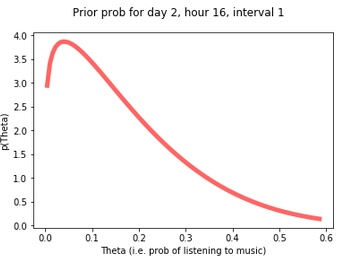
\includegraphics[width=5cm, keepaspectratio,]{fig010c.jpg}
	\caption{}
	\label{fig10c}
\end{figure} 

Here we see that the $\theta$, which represents the prior probability of listening to music in the timeslot, is most likely to be less than 0.1 for this timeslot. Note that this timeslot is for hour 17 (i.e. 5pm) which from our prelinary analysis we  know is the peak listening time. The fact that the probablity is so low suggests that users may often have weeks in which no music was played, and hence the prior probability for a timeslot is dragged down. 

For our posterior function, the threshold at which we determine a Play event was determined by comparing the false positive rates with the true positive rates using a ROC curve (\ref{fig10d}). From this, 0.4 was selected as the optimal threshold at which to determine a Play event across all users.

\begin{figure}[h!]
	\centering
	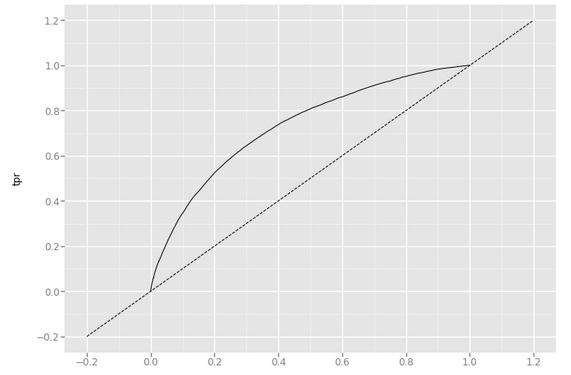
\includegraphics[width=5cm, keepaspectratio,]{fig010d.jpg}
	\caption{ROC curve showing 0.4 as the optimal threshold}
	\label{fig10d}
\end{figure} 

The results from the model are shown in figure \ref{fig10e}. We see that the recall and precision of play events (as denoted by 1) is very low suggesting that relying on a Bayesian approach centered around a weekly profile of each users habits is not an effective method for predicting a play event for a new time period.

\begin{figure}[h!]
	\centering
	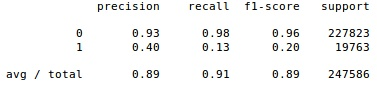
\includegraphics[width=7cm, keepaspectratio,]{fig010e.jpg}
	\caption{Beta-Bionmial Model Results}
	\label{fig10e}
\end{figure} 

\section{Logistic regression analysis}

An advantage of logistic regression over non-linear models is that the coefficients are easily interpretable. While feature engoneering was not the focus of this research an examination of these can yield insight into which features may be unecessary. 

\begin{figure}[h!]
	\centering
	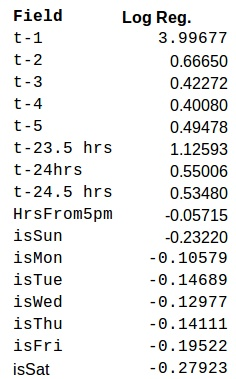
\includegraphics[width=4cm, keepaspectratio,]{fig014.jpg}
	\caption{}
	\label{fig14}
\end{figure} 

Fig \ref{fig14} shows that $t-1$ was by far the most important feature. This is expcted and it's importance crowds out the other features.

Interestingly t-23.5 is the second strongest time-lag and more significant than t-24hrs. This likely reflects the fact that having a consistent $t-1$ is more important than simply knowing what $t$ was 24 hours prior.

The non-time lag features seem to have very little effect, which was also see in fig \ref{fig16} where we do a forward stepwise regression are barely impacted by these features.

\begin{figure}[h!]
	\centering
	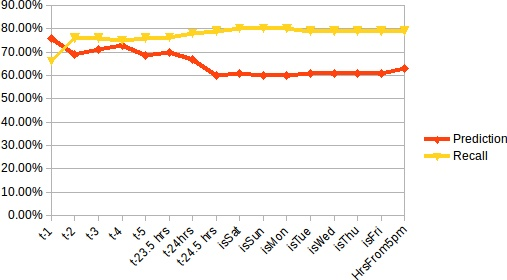
\includegraphics[width=7cm, keepaspectratio,]{fig016.jpg}
	\caption{Stepwise regression, adding in fields from left to right}
	\label{fig16}
\end{figure} 

\section{SVM analysis}

Of the two SVM models, the RBF model was selected for more in-depth analysis due to its ability to better capture recall without too detrimental a loss in precision. An RBF kernel has two hyper-paramters that can significantly impact the results. The $C$ parameter and the $gamma$. Intuitively, the gamma parameter defines how far the influence of a single training example reaches, with low values meaning ‘far’ and high values meaning ‘close’. The C parameter trades off misclassification of training examples against simplicity of the decision surface. A low C makes the decision surface smooth, while a high C aims at classifying all training examples correctly by giving the model freedom to select more samples as support vectors.

In order to determine optimal gamma and C values, a grid search was carried out with precision and recall of the test dataset plotted on a heatmap. In order to get through the many iterations of the data, the input data was reduced to 30,000 training samples. Fig \ref{fig17b} shows the final heatmap, after multiple iterations to home in on the optimal values, with precision on the left and recall on the right. The optimal values are deemed to be 0.6 for C and 0.76 for Gamma, although as the charts show there is some scope for movement around those values.

\begin{figure}[h!]
	\centering
	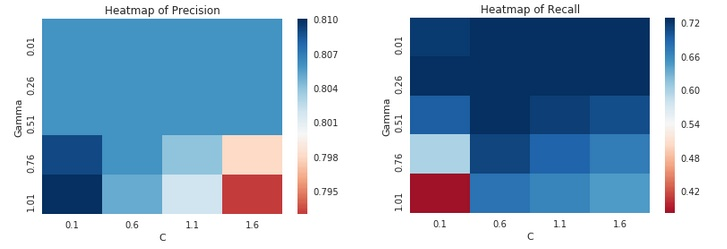
\includegraphics[width=7cm, keepaspectratio,]{fig017b.jpg}
	\caption{Heatmap of hyper-parameter search. Dark blue shade = better precision and recall}
	\label{fig17b}
\end{figure} 

Finally, a note on the computational complexity of the RBF model. We used Scikit Learn's implementation of the RBF kernel which is based on libsvm. The fit time complexity of this approach is more than quadratic with the number of samples, making it hard to scale to datasets with more than a couple of 10,000 samples \parencite{chang2011libsvm}.
While we managed to get as high as 100,000 samples in our training it was not considered a practical to go any higher thereby limiting the scalability of this approach and our ability to potentially obtain higher scores than what we already had.

\section{RNN analysis}

The RNN-LSTM model required a lot of hyper-parameter testing and as such the training dataset ended up being narrowed down to no more than 50k random samples and often as low as 20k. The eventual set of hyper-parameters that was found to work well \textit{with early stopping} were:

\begin{list}{-}{spacing}
	\item user iteration: 10 (How many random users to select for training)
	\item samplesPerUser = 20      \# How many mini-batches to select for each user
	\item batchRows = 50           \# How many random periods to select in each mini-batch (=batch height)
	\item batch iterations = 10    \# How many iterations to perform on one batch
	\item steps = 672              \# How many time steps to use (= batch depth)
	\item learning rate = 0.001    \# Learning rate of backprop algorithm
	\item Hidden units = 250       \# Number of units per hidden layer
	\item layers = 4			   \# Number of hidden layers
	\item class1Weighting = 8      \# Weighting to apply in the cost function for labels that are a play event
\end{list}

This scored an average precision of 70\% and an average recall of 66.5\% over two separate runs, with 1 run taking approximately 10 hours to complete. The original number of user iterations was 20 but a consisten pattern was that if a model runs for too long, the results swing in favour of all plays, or no plays, depending on the weighting used. Periodic testing during training and early stopping when good performance is achieved is recommended.

Fig \ref{fig15} shows the results of some of the other tests that were performed. The table has been shaded to aid understanding with darker shading what may be considered "better", whether this be more training data samples, a more complex model struture, or a better score.

\begin{figure}[h!]
	\centering
	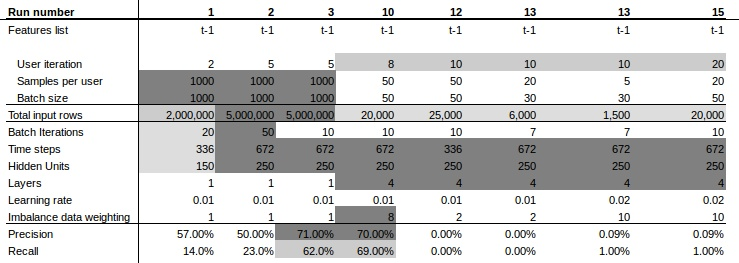
\includegraphics[width=12cm, keepaspectratio,]{fig015.jpg}
	\caption{RNN results over multiple runs. Darker shading means better}
	\label{fig15}
\end{figure}

Note that not all runs are shown - those that incorporated additional features beyond t-1 have been excluded.

\subsubsection{Hidden Layers}

We see that the improvement in precision comes about most significantly through the use of 4 layers (see run no. 7) although a higher number of iterations of a mini-batch also seems to help improve precision (see run 2 vs. 3). 

Yet too many iterations of a mini-batch adversely impacts recall. Good recall appears to be a product of a higher number of hidden units in a layer, a higher number of time steps being fed into the LSTM, and a higher number of layers. All these supports the idea that the ability to detect the start and end of a play session, requires a highly non-linear solution.
 
\subsection{Declining scores}

We also see a few results that stand out. They are runs 3, 12, and 13. Run 3 shows a reasonable score was achieved with just 1 hidden layer by performing fewer mini-batch iterations than run 2. While runs 12 and 13 showed a score of 0\% by the end of their runs.

Both of these are attributed to an observation that the longer the model is trained the more likely it is to start predicting 'not a play event' for everything. We hypothesized that this is due to the data imbalance, which in over many training iterations leads the model to conclude getting the non-play events correct is more important than getting the play events correct.






We see this better in fig \ref{fig18a} which shows the precision and recall of every minibatch sample. Note that in this chart, every 50 mini-batches represents the end of a random user, before another one is randomly selected. Fig. \ref{fig18a} shows us both the scores of each mini-batch training data (lighter colored markers), as well as the scores at the end of each random user, using randomly selected test data (darker symbols).

\begin{figure}[h!]
	\centering
	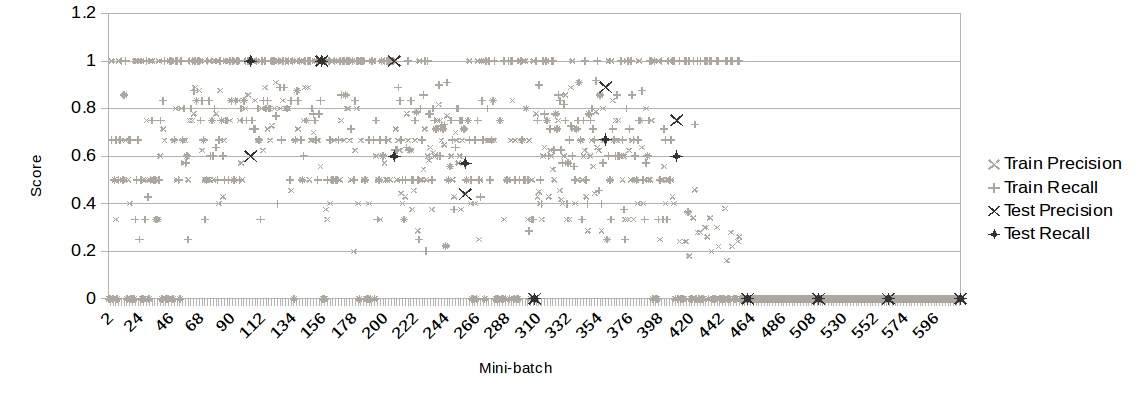
\includegraphics[width=12cm, keepaspectratio,]{fig018a.jpg}
	\caption{RNN results over multiple runs. Darker shading means better}
	\label{fig18a}
\end{figure}

\begin{figure}[h!]
	\centering
	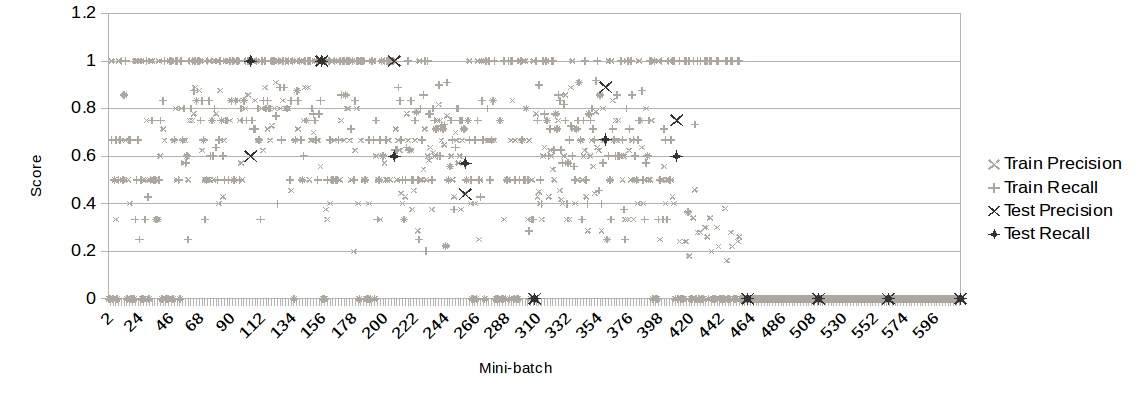
\includegraphics[width=12cm, keepaspectratio,]{fig018a.jpg}
	\caption{RNN results over multiple runs. First 100 rows.}
	\label{fig18b}
\end{figure}

Note that it is generally easier to achieve a high precision score by only guessing play events infrequntly, resulting in a lower recall score; and that in each mini-batch, less than 10\% of rows would be a 'play event'. 

From loking at fig. \ref{fig18a} it is hard to discern whether there are any patterns. For this reason we also include fig. \ref{fig18b} showing just the first 100 rows.

There are two insights we draw from these charts:
\begin{enumerate}
	\item It is hard to tell if results are improving with each mini-batch however we do see in fig. \ref{fig18b} that there are fewer scores of 0\% as training goes on.
	\item After a certain point in training results fall off a cliff edge -- the model predicts 'No play' for every event
\end{enumerate}
 



Finally, an RNN-LSTM model has a computational complexity of per time-step and weight of O(1) \parencite{gers1999learning}. While training still took some time, with better hardware applying the method to ever larger datasets is not intractable.